\chapter{Let's Get Started}
\label{ch:lgstarted}
% ##################################################################################################################
\hfill \textbf{Authors:} Marcel Rieser, Andreas Horni, Kai Nagel

\begin{center} 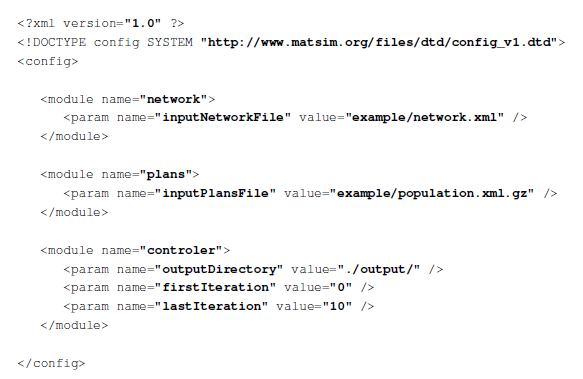
\includegraphics[width=0.7\textwidth, angle=0]{using/figures/config.png} \end{center}

\editdone{This text has undergone the professional edit. Please no grammatical changes anymore! They are most-probably wrong.}

% ##################################################################################################################
This chapter explains how to set up and run \gls{matsim} and describes the requirements for building a basic \gls{scenario}.  Updated information may be available from \url{http://matsim.org}, in particular from \url{http://matsim.org/docs}.

%% This book attempts to be as stable and timely as possible, meaning that the \gls{matsim} user guide \citep[][]{MATSim_Userguide_2015} \todokai{rm usrguide} should also be consulted when doing an actual installation. Frequently changed, detailed information like download paths, or version-dependent configurations, are omitted here---as far as possible---and left to the user guide. 

Getting the source code into different computing environments and extending \gls{matsim} through the \gls{api} is described in the book's second part, Chapter~\ref{ch:extensionpoints}.

%% \kai{Ich würde bei den xml snippets gerne überall den header entfernen, überall eine Formulierung benuzten in etwa wie ``a minimal config file approximately looks as follows'', und überall zusätzlich eine stabile(!!) Referenz auf Versionen im Repository geben (muss noch schauen, wie wir das machen).  Z.B.\ ist config inzwischen bereits v2, und hat an manchen Stellen eine modernere Syntax; das fällt nur deshalb nicht auf, weil die alte Syntax noch überall akzeptiert wird.}

%% \ah{klingt gut.}

% ##################################################################################################################
\section{Running MATSim}
\label{sec:runningmatsim}

% ================================================================================================
\subsection{Setting Up MATSim}
\label{sec:settingUpMatsim}

To run \gls{matsim} you must install the \gls{javase} that complies with the appropriate \gls{matsim} version. At this time, this is \gls{javase}~7.

You also need the official \emph{\gls{matsim} release,} a zip file (usually designated with the version number \lstinline|matsim-yy.yy.yy.zip|), that includes everything required to run it. It can be downloaded following the ``release'' link under \url{http://matsim.org/downloads}.
%on the \gls{matsim} web page. 
Unzipping results in the \textbf{\gls{matsim} directory tree}. Continue with Section~\ref{sec:runexample}.

If you prefer to use the more up-to-date---but less stable---\emph{nightly builds,} you should download, via the same \gls{url} \url{http://matsim.org/downloads},
\begin{itemize}\styleItemize
\item the \gls{matsim} \gls{jar} file (usually tagged with the revision number \lstinline|MATSim_ryyyy.jar|), and
\item the required external \glspl{library} (\lstinline|MATSim_libs.zip|). 
Unzipping this collection of 3rd-party libraries, you should then get a directory \lstinline|libs|, with several \gls{jar} files inside. If the directory \lstinline|libs| is in the same directory as the \gls{matsim} \gls{jar} file, the libraries are found automatically and don't have to be added manually to the \lstinline|classpath|.
\end{itemize}
Continue with Section~\ref{sec:runexample}.

% ================================================================================================
\subsection{Running MATSim}
\label{sec:runexample}
When this book was written, the nightly built \gls{matsim} \gls{jar} file was executed by double-clicking. A minimal \gls{gui}, as shown in Figure~\ref{fig:matsimgui}, opens and the \gls{matsimrun} can be configured and started. 
This feature will appear in the releases, starting with version~0.8.
%
% ----------
\createfigure[!h!]%
{Minimal MATSim GUI}%
{Minimal MATSim GUI}%
{\label{fig:matsimgui}}%
{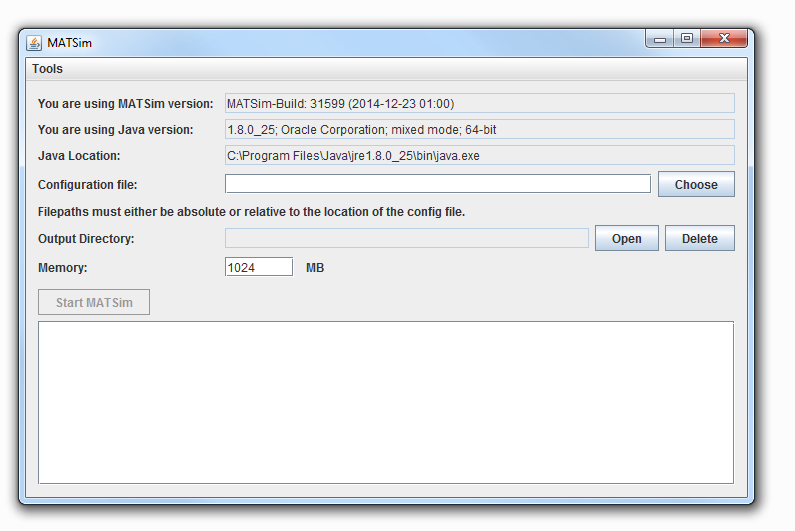
\includegraphics[width=0.8\textwidth, angle=0]{using/figures/matsimgui.png}}%
{}
% ----------

For the release~0.6, \gls{matsim} does not provide a \gls{gui}; thus, you must be able to handle and access a command line tool.
%\footnote{%
%%
%\parskip0.3\baselineskip
%\parindent0pt
%
In \gls{linux} or \gls{mac} OS X, this is typically a Terminal application; in \gls{windows}, the Power Shell or Command Prompt.
%
On the command prompt type the following command in one line, but substitute the correct paths: 
%% \lstinline|java -Xmx512m -cp /path/to/matsim.jar org.matsim.run.Controler /path/to/config.xml|

On Linux or Mac OS X, something like:
\begin{shell}
java -Xmx512m -cp /path/to/matsim.jar org.matsim.run.Controler /path/to/config.xml
\end{shell}

%% On Mac OS X: 
%% \lstinline|java -Xmx512m -cp /path/to/matsim.jar org.matsim.run.Controler /path/to/config.xml|

On Windows, an example command could be: 
\begin{shell}
java -Xmx512m -cp C:\MATSim\matsim.jar org.matsim.run.Controler
   C:\MATSim\input\config.xml
\end{shell}
%% \begin{lstlisting}
%% java -Xmx512m -cp C:$\backslash$MATSim$\backslash$matsim.jar org.matsim.run.Controler
%%    C:$\backslash$MATSim$\backslash$input$\backslash$config.xml
%% \end{lstlisting}
% problems with the combination of lstinline, backslash, and footnote. :-(  kai, jan'15
%\ah{... and linebreaks ... and \begin{lstlisting}}

Such a command consists of multiple parts:
\begin{itemize}\styleItemize
\item \lstinline|java| tells the system that you want to run \gls{java}.
\item \lstinline|-Xmx512m| tells \gls{java} that it should use up to 512\,\gls{mb} of memory. This is typically enough to run the small examples. For larger \glspl{scenario}, you might need more memory, \eg \lstinline|-Xmx3g| would allow \gls{java} to use up to 3\,\gls{gb} of \gls{ram}.
\item \lstinline|-cp /path/to/matsim.jar| tells Java where to find the \gls{matsim} code.
\item \lstinline|org.matsim.run.Controler| specifies which class (think of an ``entry point'') should be run. In most cases, the default \gls{matsim} \lstinline|Controler| is the class you will need to run simulations.
\item \lstinline|/path/to/config.xml| tells \gls{matsim} which \gls{configfile} is to be used. 
\end{itemize}
%}

% ================================================================================================
\subsection{Configuring \protect\gls{matsim}}
\label{sec:lgs-config}
 \gls{matsim} is configured 
%(at this stage) only 
% KISS.  kai, jan'15
 in the \gls{configfile}, building the connection between the user and \gls{matsim} and containing a settings list that influences how the simulation behaves.
%% In the second part of the book we will learn how \gls{matsim} can be configured and extended by programming against its API. \kai{Andreas, hier brauchen wir eine Entscheidung.  Derzeit enthält ``extending matsim'' auch Material, welches alleine durch die Config angesprochen werden kann, ohne contrib und ohne programming.  Beispiele sind time-dep network, andere strategy modules, oder observational modules.  Mit ``transit'' wird das nochmal deutlich mehr.  Nichts davon ist somit ``programming against its API''.  Möglichkeiten aus meiner Sicht: 
% (1) Wir verstehen unter ``extending'' auch solche Dinge, die alleine durch die config (und evtl. zusätzliche Input-Dateien) angesprochen werden können.  
% (2) Wir packen Dinge, die über die config ansprechbar sind, aber zusätzliche Dateien benötigen, nach ``extending'', alles andere nach ``using''.  
% (3) Wir packen \emph{nur} die Dinge, bei denen man programmieren muss, nach ``extending''. --  Im Moment ist es m.E.\ (1).  -- Wenn es (1) oder (2) sind/werden, müsste man obigen Satz anpassen.}
%
%\kai{Habe einen Satz, der eine Vorschau auf Part~II gibt, mal rausgestrichen.  Part~II enthält auf jeden Fall auch (viele) Dinge, die man machen kann, ohne dass man programmiert.}
%\ah{Die nur grob definierte Einteilung machte mir im Modules-Chapter auch schon grosse Bauchschmerzen.
%
%Grundidee war mal (3). Doch dann landet viel zu viel, was den Anfänger überfordert in Teil I. Das Modules-Kapitel müsste komplett auseinandergerissen werden.
%(1) ist noch keine klare Grenze, was wir im Moment ja auch nicht haben. 
%So was wie (2) müsste es m.E. sein, um eine didaktisch sinnvolle Einteilung zu haben. Aber auch hier, muss das Modules-Kapitel auseinandergerissen werden. Wir sollten wohl noch ein Using-Kapitel einfügen mit dem Titel "Configuring MATSim" o.ä., und da alles reinpacken, was momentan im Modules-Kapitel nur über Config angesprochen werden kann.
%} \ah{Kaüitel eingefügt}

All configuration parameters are simple pairs of a parameter \lstinline|name| and a parameter \lstinline|value|. The parameter are grouped into logical groups; one group has settings related to the \lstinline|Controler|, like the number of \glspl{iteration}, or another group has settings for the \gls{simulation}, \eg end time of the simulation. As shown in Chapter~\ref{ch:modules}, numerous \gls{matsim} modules can be added to \gls{matsim} and configured by specifying the respective configuration file section.

The list of available parameters and valid parameter values may vary from release to release. Although we try to keep this stable,
%due to
software changes, mainly new features, may cause settings to change. For a list of all available settings available with the version you are working with, run the following command:
\begin{lstlisting}
java -cp /path/to/matsim.jar org.matsim.run.CreateFullConfig fullConfig.xml
\end{lstlisting}
%
This command will create a new \gls{configfile} \lstinline|fullConfig.xml|, containing all available parameters--along with their default values, making it easy to see what settings are available. To use and modify specific settings, lines with their corresponding parameters can be copied to the \gls{configfile}, specific to the \gls{scenario} to be simulated and the parameter values to be modified in that file. 

A fairly minimal \gls{configfile} contains the following information:
\begin{xml}
<module name="network">
   <param name="inputNetworkFile" value="<path-to-network-file>" />
</module>

<module name="plans">
   <param name="inputPlansFile" value="<path-to-plans-file" />
</module>

<module name="controler">
   <param name="firstIteration" value="0" />
   <param name="lastIteration" value="0" />
</module>

<module name="planCalcScore" >
   <parameterset type="activityParams" >
      <param name="activityType" value="h" />
      <param name="typicalDuration" value="12:00:00" />
   </parameterset>
   <parameterset type="activityParams" >
      <param name="activityType" value="w" />
      <param name="typicalDuration" value="08:00:00" />
   </parameterset>
</module>
\end{xml}
For a working example, see the \gls{matsim} directory tree (\cf \ref{sec:settingUpMatsim}) under \lstinline{examples/tutorial/config/example1-config.xml}.
 
In the example, supply is provided 
by the network and demand by the plans file. Typical input data is described in Section~\ref{sec:inputdata}. 
%
The specification that the first and last iteration are the same means that no \gls{replanning} of the demand is performed.  
%
What \emph{is} executed is the \gls{mobsim} (Figure~\ref{fig:matsimcycle}), followed by each executed plan's performance scoring.
%
To function, the scoring needs to know, from the \gls{configfile}, all activity types used in the plans and the typical duration for each activity type.

Further configuration possibilities are described in Chapter~\ref{ch:configuring}.

% ##################################################################################################################
\section{Building and Running a Basic Scenario}
\label{sec:buildingbasicscenario}
% ===============================================================================================
This section provides information on typical input data files used for a \gls{matsim} experiment, as well as the standard output files generated. It presents a minimal example scenario and briefly explains units, conventions and coordinate systems used in \gls{matsim}. Then, hints on practical data requirements
% and how to perform calibration, verification and validation 
are provided.

% ===============================================================================================
\subsection{Typical Input Data}
\label{sec:inputdata}
Minimally \gls{matsim} needs the files
\begin{itemize}\styleItemize
	\item \lstinline|config.xml|, containing the configuration options for \gls{matsim} and presented above,
	\item \lstinline|network.xml|, with the description of the (road) network, and
	\item \lstinline|population.xml|, providing information about travel demand, \ie list of agents and their day plans.
\end{itemize}

%% \kai{Andreas, eigentlich würde ich `facilities', `vehicles', und `transit' gerne nach ``extending matsim'' verschieben: (1) `facilities' kann man nur mit core matsim und config file m.E. gar nicht benutzen, (2) schedule-based pt ist ein fehler-anfälliger plug-in, mit dem man nicht gleich ``starten'' muss.  Ok?} \ah{ok}
%% \kai{clean this out (facilities, pt, etc.} \ah{done}

\lstinline|population.xml| and \lstinline|network.xml| 
% or \lstinline|facilities.xml| \kai{chk if already known here}, \ah{cleaned}
might get quite large. To save space, \gls{matsim} supports reading and writing data in a compressed format. \gls{matsim} uses GZIP-compression for this. Thus, many file names have the additional suffix \lstinline|.gz|, as in \lstinline|population.xml.gz|. \gls{matsim} acknowledges whether files are compressed, or should be written compressed, based on file name.

% --------------------------------------------------------------------
\subsubsection{An Outlook to Extending MATSim in Part II of this Book}
Section~\ref{sec:extending:initial-input} provides some information about \gls{matsim}'s technical tools for initial input generation.
With the basic setting, \gls{matsim} agents perform their activities on a specific \gls{link}. If further information about \glspl{activitylocation} needs to be specified, this can be carried out with facilities described in Section~\ref{sec:extending-facilities}. Further, for the \emph{simulation} of public transport, the base scenario must be extended by additional files as shown in Section~\ref{sec:inputdata:transitvehicles} and Chapter~\ref{ch:pt}. Count data are a common evaluation measure in transport planning. In \gls{matsim}, count data can be provided for the simulation, as shown in Section~\ref{sec:extending-counts}. 
 
In more detail, the network and population files resemble the following; for the \gls{configfile}, see Section~\ref{sec:lgs-config} above.

\makeatletter
\newcommand\thefontsize{{The current font size is: \f@size pt\par}}
\makeatother

% -----------------------------------------------------------------------
\subsubsection{\lstinline{network.xml}}
\label{sec:lgstarted-network-file}
 Network is the infrastructure on which agents (or vehicles), can move around. The network consists of \glspl{node} and \glspl{link} (in graph theory, typically called vertices and edges). A simple network description in \gls{matsim}'s \gls{xml} data format 
could contain approximately the following information:
%% <?xml version="1.0" encoding="utf-8"?> 
%% <!DOCTYPE network SYSTEM "http://www.matsim.org/files/dtd/network_v1.dtd"> 
\begin{xml}
<network name="example network"> 
   <nodes> 
      <node id="1" x="0.0" y="0.0"/> 
      <node id="2" x="1000.0" y="0.0"/> 
      <node id="3" x="1000.0" y="1000.0"/> 
   </nodes> 
   <links> 
      <link id="1" from="1" to="2" length="3000.00" capacity="3600" 
            freespeed="27.78" permlanes="2" modes="car" /> 
      <link id="2" from="2" to="3" length="4000.00" capacity="1800" 
            freespeed="27.78" permlanes="1" modes="car" /> 
      <link id="3" from="3" to="2" length="4000.00" capacity="1800" 
            freespeed="27.78" permlanes="1" modes="car" /> 
      <link id="4" from="3" to="1" length="6000.00" capacity="3600" 
            freespeed="27.78" permlanes="2" modes="car" /> 
   </links> 
</network>
\end{xml}
For a working example, check the \lstinline{examples/equil} directory in the \gls{matsim} directory tree (\cf Section~\ref{sec:settingUpMatsim}).

Each element has an identifier \lstinline|id|. Nodes are described by an \lstinline|x| and a \lstinline|y| coordinate value. Links have more features; the \lstinline|from| and \lstinline|to| attribute reference nodes and describe network geometry. Additional attributes describe traffic-related link aspects:
%network:
\begin{itemize}\styleItemize
    \item the \lstinline|length| of the link, typically in meters (see Section~\ref{sec:unitsconventions}).
    \item the flow \lstinline|capacity| of the link, \ie number of vehicles that traverse the link, typically in vehicles per hour.
    \item the \lstinline|freespeed| is the maximum speed that vehicles are allowed to travel along the link, typically in meters per second.
    \item the number of lanes (\lstinline|permlanes|) available in the direction specified by the 'from' and 'to' nodes.
    \item the list of \lstinline|modes| allowed on the link. This is a comma-separated list, \eg \lstinline|modes="car, bike, taxi"|.
\end{itemize}
%Note that
All links are uni-directional. If a road can be traveled in both directions, two links must be defined with alternating \lstinline|to| and \lstinline|from| attributes (see links with id~2 and 3 in the listing above). Then, the network can be seen as a directed graph. 

% -----------------------------------------------------------------------
\subsubsection{\lstinline|population.xml|}
\label{sec:lgstarted-population-file}
% ........................................................
\paragraph{File Format}

 \gls{matsim} travel demand is described by the agents' day plans. The full set of agents is also normally defined as the population, hence the file name \lstinline|population.xml|. Alternatively, \lstinline|plans.xml| is also commonly used in \gls{matsim}, as the population file essentially contains a list of day plans.

The population contains the data in a hierarchical structure, as shown in the following example.  This example illustrates the data structure; minimal input files need less information, as illustrated later.
%% <?xml version="1.0" encoding="utf-8"?> 
%% <!DOCTYPE population SYSTEM "http://www.matsim.org/files/dtd/population_v5.dtd"> 
\begin{xml}
<population> 
   <person id="1"> 
      <plan selected="yes" score="93.2987721"> 
         <act type="home" link="1" end_time="07:16:23" /> 
         <leg mode="car"> 
            <route type="links">1 2 3</route> 
         </leg> 
         <act type="work" link="3" end_time="17:38:34" /> 
         <leg mode="car"> 
            <route type="links">3 1</route> 
         </leg> 
         <act type="home" link="1" /> 
      </plan> 
   </person> 
   <person id="2"> 
      <plan selected="yes" score="144.39002"> 
         ...
      </plan> 
   </person> 
</population>
\end{xml}
For a working example, check the \lstinline{examples/equil} directory in the \gls{matsim} directory tree (\cf Section~\ref{sec:settingUpMatsim}).

The population contains a list of persons, each person contains a plan list and each plan contains a an activities and legs list.

Exactly one \gls{plan} per person is marked as selected. Each agent's selected plan is executed by the mobility simulation. During the \gls{replanning} stage, a different plan might be marked as selected. A \gls{plan} can contain a score as attribute. The score is calculated and stored in the plan after its execution by the mobility simulation during the scoring stage.

The list of activities and legs in each plan describe each agent's planned actions. Activities are assigned  a type and have---except for the last activity in a day plan---a defined end time. There are some exceptions, where activities have a duration instead of an end time. Such activities are often automatically generated by routing algorithms and are not described in this book. To describe the location where an activity takes place, the activity is either assigned a coordinate by giving it an \lstinline|x| and \lstinline|y| attribute value, or it has a link assigned, describing from which link the activity can be reached. Because the simulation requires a link attribute, \lstinline|Controler| calculates the nearest link for a given coordinate, for a missing attribute; only a \lstinline|x| and \lstinline|y| coordinate value is given for any activity.

A \gls{leg} describes how agents plan to travel from one location to the next; each \gls{leg} must have a transport mode assigned. Optionally, legs may have an attribute, \lstinline|trav_time|, describing expected travel time for the leg. For a leg to be simulated, it must contain a route. The format of a route depends on the mode of a leg. For car-legs, the route lists the links the agent has to traverse in the given order, while for transit-legs, information about stop locations and expected transit services are stored.

An agent starts a leg directly after the previous activity (or leg) has ended. Depending on the mode, the \gls{mobsim} might handle the agent differently. By default, car- and transit-legs are well-supported by the \gls{mobsim}. If the \gls{mobsim} encounters a mode it does not know, it defaults to \gls{teleportation}. In this case, an agent is removed from the simulated reality and re-inserted at its target location after the leg's expected travel time has passed.

% ........................................................
\paragraph{A Minimal Population File}

The population data format is one of the most central data structures in \gls{matsim} and might appear a bit overwhelming at first. Luckily, to get started, it is only necessary to know only a small subset.  A population file needs, approximately,  the following information:
%% This listing shows what a minimal population file could look like. 
%% <?xml version="1.0" encoding="utf-8"?> 
%% <!DOCTYPE population SYSTEM "http://www.matsim.org/files/dtd/population_v5.dtd"> 
\begin{xml}
<population> 
   <person id="1"> 
      <plan> 
         <act type="home" x="5.0" y="8.0" end_time="08:00:00" /> 
         <leg mode="car" /> 
         <act type="work" x="1500.0" y="890.0" end_time="17:30:00" /> 
         <leg mode="car" /> 
         <act type="home" x="5.0" y="8.0" /> 
      </plan> 
   </person> 
   <person id="2"> 
      ... 
   </person> 
</population>
\end{xml}
For a working example, check the \lstinline{examples/equil} directory in the \gls{matsim} directory tree (\cf Section~\ref{sec:settingUpMatsim}).

The following items can be simplified:
\begin{itemize}\styleItemize
\item Each person needs exactly one plan.
\item The plan does not have to be selected, or have a score.
\item Activities can be located just by their coordinates.
\item Activities should have a somewhat reasonable end-time.
\item Legs need only a mode, no routes.
\end{itemize}
When a simulation is started, \gls{matsim}'s \lstinline|Controler| will load such a file and then automatically assign the link nearest to each activity and calculate a suitable route for each leg. This makes it easy to get started quickly. 

% ===============================================================================================
\subsection{Typical Output Data}
\label{sec:outputdata}
\gls{matsim} creates
% significant
output data, which can be used to analyze results, but also to monitor the current simulation setup's progress. Some of the files summarize a complete \gls{matsimrun}, while others are created for a specific \gls{iteration} only. The first files go directly to the output folder's top level, which can be specified in the \lstinline|controler| section of the \gls{configfile}. The other files are stored in iteration-specific folders \lstinline|ITERS/it.{iteration number}|, continuously created in the output folder. For some files (typically for  large ones, such as population), output frequency can be specified in the \gls{configfile}. They go to the respective iteration folder. The files summarizing the complete \gls{matsimrun} are built on the fly, \ie after every iteration, currently computed iteration values are stored, allowing continuous monitoring of the run. Some files are created by default (such as the score statistics files); others need to be triggered by a respective configuration file section (such as count data files).

%\kai{Sollten wir (1) den Unterschied zwischen ``main'' und ``ITERS'' directory beschreiben, und (2) darauf hinweisen, wo die folgenden Dateien jeweils sind?}
%\ah{sollte jetzt erledigt sein}

The following output files are continuously built up to summarize the complete run.
\begin{description}\styleDescription

  \item[Log File:]
During a \gls{matsimrun}, a log file is printed containing information you might need later for your analyses, or in case a run has crashed, for any reason. 

\item[Warnings and Errors Log File:]
Sometimes, \gls{matsim} identifies problems in the simulation or its configuration; it will then write warning and error messages to the log file. Because the log file contains so much information, these warnings can be overlooked. For this reason, a separate log file is generated in a run output directory, containing only warnings and error messages. It is important to check this file during/after a run for updates on any major problems.

\item[Score Statistics:]
Score statistics are available as picture (\lstinline|scorestats.png|), as well as a text file (\lstinline|scorestats.txt|). They show the average best, worst, executed and overall average of all an agent's plans for every iteration. An example score plot is shown in Figure~\ref{fig:scoreprogress}.

\item[Leg Travel Distance Statistics:]
Leg travel distance statistics (files \lstinline|traveldistancestats.png| and \lstinline|traveldistancestats.txt|) are comparable to score statistics, but instead, they plot travel distance. 

\item[Stopwatch:]
The stopwatch file (\lstinline|stopwatch.txt|) contains the computer time (so-called wall clock time) of actions like replanning or execution of mobility simulation for every iteration. This data might be helpful for performance analyses (\eg how long does replanning take compared to the mobility simulation?).

\end{description}

%\kai{``run'' vs ``iterations'': Wir benutzen normalerweise die Semantik, dass ein ``run'' die Summe aller ``iterations'' ist.  Dann wäre das oben ``Once per iteration''.  Oder ``At the end of each run'', obwohl das technisch nicht richtig ist, weil es tatsächlich am Ende einer jeden Iteration neu erzeugt wird; so kann man alles bereits während der Iterationen mitverfolgen.}
%\ah{sollte jetzt erledigt sein}

The following output files are created for specific iterations:
\begin{description}\styleDescription

\item[Events:] Every action in the simulation is recorded as a so-called \gls{matsim} \gls{event}, be it an activity start or change of network link. Each \gls{event} hosts one or multiple attributes. By default, the time when the \gls{event} occurred is included. Additionally, information, like the ID of the agent triggering the event, or the link ID where the \gls{event} occurred, could be included. Also by default, the \gls{matsim} simulation module creates a so-called events file in every 10th iteration, containing every \gls{event}  created by the simulation. The events file is thus an important base for post-analyses, like the visualizers. Events are discussed in detail in Section~\ref{sec:events-extension-point}.

\item[Plans:] At configurable iterations, the current state of the population, with the agents' plans, is printed.
%
Final iteration's plans 
%and events % nicht per default. kai, jan'15
are also generated on the top level of the output folder.

\item[Leg Histogram:]
In every iteration, a leg histogram is plotted. A leg histogram depicts the number of agents arriving, departing or en route, per time unit. Histograms are created for each transport mode and for the sum of all transport modes. Each file starts with the iteration number and ends with the transport mode (\eg \lstinline|1.legHistogram_car.png| or \lstinline|1.legHistogram_all.png|). A text file is also created (\eg \lstinline|1.legHistogram.txt|), containing the data for all transport modes.

\item[Trip Durations:]
For each iteration, a \gls{trip} durations text file (\eg \lstinline|1.tripdurations.txt|), listing number of trips and their durations---on a time bin level for each activity pair (\eg from work to home or from home to shopping)---is produced.

\item[Link Stats:] In each iteration, a link stats file containing hourly count values and travel times on every network link is printed. Link stats are particularly important for comparison with real-world count data, as introduced in Section~\ref{sec:extending-counts}.

%\item[Link Volumes:]
%The printing of the link volume comparison (between simulated and counted volumes) needs to be triggered by a config file entry. 
%\ah{This has to be in the extending part. Moved figure and some text there}
%
\end{description}

% ===============================================================================================
\subsection{An Example Scenario}
The \gls{matsim} release is shipped with an example scenario named \lstinline|equil| in the folder \lstinline|examples/equil|, containing these files: \lstinline|config.xml|, \lstinline|network.xml|, \lstinline|plans100.xml|, and \lstinline|plans2000.xml.gz|, containing, respectively, 100 and 2000\,persons with their day plans, using car mode only. A tiny population containing only 2\,persons (\lstinline|plans2.xml|), one using public transport, the other using car mode, is also provided. An example for count data is also found in the folder (\lstinline|counts100.xml|). 

%% or trips with taxi mode is also provided (\lstinline|plans-w-taxi.xml|). 
%% A tolls file can be used for road pricing scenarios not discussed here (\lstinline|toll.xml|).

%\kai{Habe da neulich, als Resultat einer Diskussion, etwas ausgedünnt.  Müssen wir ggf.\ anpassen, aber m.E.\ stimmt es so nun.}
%\ah{https://matsim.atlassian.net/browse/MATSIM-286}

One file also exists, with a demand of 
%exactly 
% KISS.  kai, jan'15
100~\emph{trips} (\lstinline|plans100trips.xml|), \ie demand going only from one location to another, using a \lstinline$dummy$ activity type at each end.  This is provided to show that \gls{matsim} can also be run as a fully trip-based approach,without considering any activities. Clearly, it loses some of its expressiveness, but the basic concepts, including route and even departure time adaptation, still work in exactly the same way.

The scenario network is shown in Figure~\ref{fig:equil}.
%
% ----------
\createfigure%
{Equil scenario network}%
{Equil scenario network}%
{\label{fig:equil}}%
{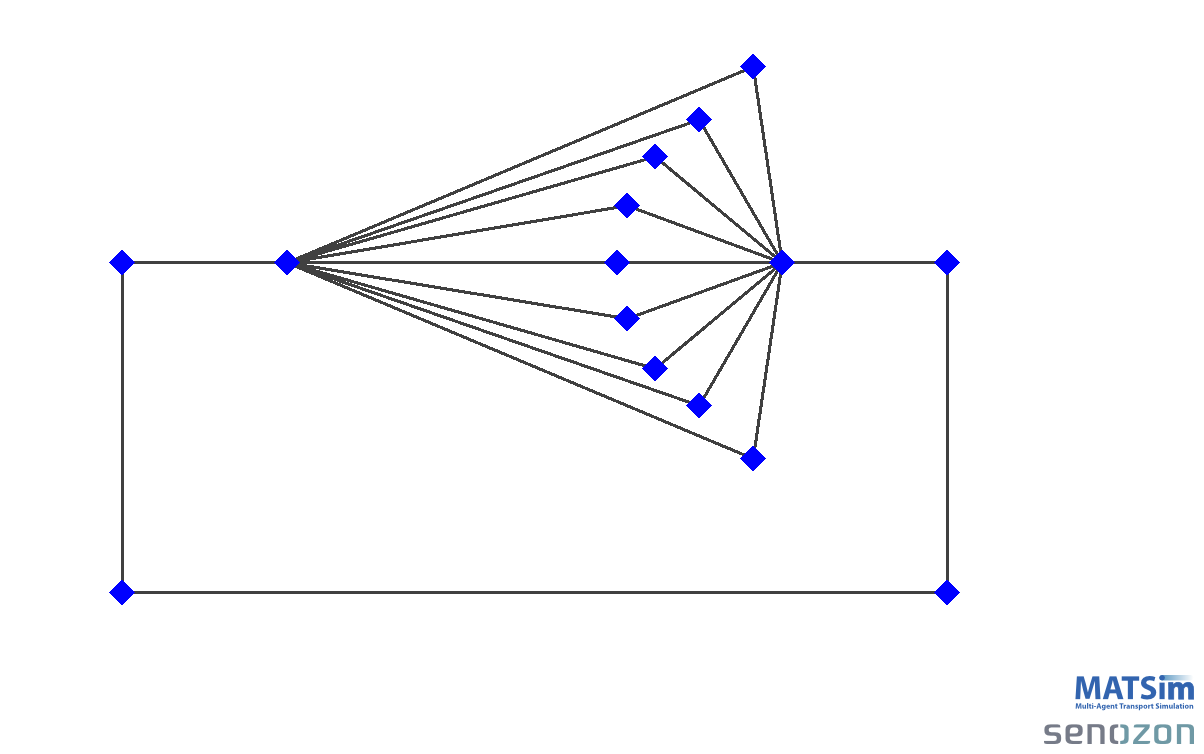
\includegraphics[width=0.8\textwidth, angle=0]{using/figures/equil.png}}%
{}
% ----------

The following lines explain the scenario by picking and discussing most important sections from the \gls{configfile} \lstinline|config.xml|.


\paragraph{"strategy" Section of the \protect\gls{configfile}}

As shown below, this scenario uses replanning. 10\,\% of the agents reroute their current route (module \lstinline|ReRoute|). The remaining 90\,\% select their highest score plan for re-execution in the current iteration (module \lstinline|BestScore|). Plans are deleted from the agent's memory if it is full, defined by \lstinline|maxAgentPlanMemorySize|. By default, the plan with the lowest score is removed, while this is configurable and currently being
%intense % kein funding. kai, jan'15
researched (see Section~\ref{sec:choicesets}).
%
\begin{xml}
<module name="strategy">
   <param name="maxAgentPlanMemorySize" value="5" /> <!-- 0 means unlimited -->

   <parameterset type="strategysettings" >
      <param name="strategyName" value="SelectExpBeta" />
      <param name="weight" value="0.9" />
   </parameterset>

   <parameterset type="strategysettings" >
      <param name="strategyName" value="ReRoute" />
      <param name="weight" value="0.1" />
   </parameterset>
</module>
\end{xml}


%% \kai{I think there is a better syntax for the above now (without the numbering); should we use that?}
%% \ah{ersetzt}

\paragraph{"planCalcScore" Section of the \protect\gls{configfile}}

The section \lstinline|planCalcScore| defines parameters used for scoring, explained in Chapter~\ref{ch:scoring}. As seen in the example, the two activity types \lstinline|h| (home) and \lstinline|w| (work), are specified.  All activity types contained in the population file (\cf Section~\ref{sec:lgstarted-population-file}) must be defined in the \lstinline{planCalcScore} section of the \gls{configfile}.
\begin{xml}
<module name="planCalcScore" >
   <parameterset type="activityParams" >
      <param name="activityType" value="h" />
      <param name="typicalDuration" value="12:00:00" />
   </parameterset>
   <parameterset type="activityParams" >
      <param name="activityType" value="w" />
      <param name="typicalDuration" value="08:00:00" />
   </parameterset>
</module>
\end{xml}

\paragraph{"controler" Section of the \protect\gls{configfile}}

The scenario is run for 10\,iterations, writes the output files to \lstinline|./output/equil| (Section~\ref{sec:outputdata}) and uses \gls{qsim} as the \gls{mobsim} (more on \glspl{mobsim} in Section~\ref{sec:trafficflowmodel}, \ref{sec:using-mobsims} and \ref{sec:extending-qsim}).
\begin{xml}
<module name="controler">
   <param name="outputDirectory" value="./output/equil" />
   <param name="lastIteration" value="10" />
   <param name="mobsim" value="qsim" />	
</module>
\end{xml}

%% \kai{I would suggest to say something about via already at this point.  There is a free educational version so I think that this would be ok.}
%% \ah{ok}

\paragraph{Visualization}

Simulation results can be comfortably analyzed, using one of the visualizers, \gls{via} (Chapter~\ref{ch:via}) or \gls{otfvis} (Chapter~\ref{ch:otfvis}).

% ===============================================================================================
\subsection{Units, Conventions, and Coordinate Systems}
\label{sec:unitsconventions}
% ----------------------------------------------------------------------------
\subsubsection{Units}
\gls{matsim} tries to make as few assumptions about actual units as possible, but it is sometimes necessary to estimate. In general, \gls{matsim} expects similar values (\eg all distances) to be in the same unit wherever they are used. In the following short overview, the most important (expected) units are listed.

% .......................................................
\paragraph{Distance}

Distance units are most often used in links' length. They should be specified in the same unit the coordinate system uses, allowing \gls{matsim} to use simple triangulation, \eg with the nodes' coordinates, to calculate beeline distances. As most projected coordinate systems (see Section~\ref{sec:coordinatesystems}) use meters as unit of distance, this is the most commonly used distance unit in \gls{matsim}. 

% .......................................................
\paragraph{Time}

 \gls{matsim} supports an hour:minute:second notation in several places, but internally,it uses seconds as the default time unit. This implies, for example, that link speeds must be specified in distance per second, typically meters per second. One notable exception to this rule are scoring parameters, where \gls{matsim} expects values per hour; most behavioral parameters, like value of time, are typically estimated per minute or hour, and corresponding values for seconds are very small and thus error prone. 

% .......................................................
\paragraph{Money}

Money is unit-free. Units are implicitly given by the marginal utility of money (\cf Equation~(\ref{eq:tdisutility}) below). Thus, when one moves from Germany to Switzerland, the parameter $\beta_c$ must be changed from ``utility per Euro'' to ``utility per Swiss Franc''.

% ----------------------------------------------------------------------------
\subsubsection{Conventions}
\gls{matsim} uses identifiers, short \lstinline|Id|s, intensely. These identifiers can be arbitrary strings, with the following exceptions: IDs should contain no spaces (incl. tabs, new lines, etc) or commas, because those characters are typically used for separating different IDs from each other on \lstinline|Id| lists. 

% ----------------------------------------------------------------------------
\subsubsection{Coordinate Systems}
\label{sec:coordinatesystems}
\paragraph{Preparing Your Data in the Appropriate Coordinate System}
In several input files, you need to specify coordinates, \eg for network nodes. We strongly advise not to use WGS84 coordinates (\ie \gls{gps} coordinates), or any other spherical coordinates (coordinates ranging from $-180$ to $+180$ in west-east direction and from $-90$ to $+90$ in south-north direction). \gls{matsim} has to calculate distances between two points in several sections of the code. Calculation of distances between spherical coordinates is very complex and potentially slow. Instead, \gls{matsim} uses the simple Pythagoras' theorem, but this requires Cartesian coordinate system coordinates. Thus, we emphatically recommend using a Cartesian coordinate system along with \gls{matsim}, preferably one where the distance unit corresponds to one meter.

Many countries and regions have custom coordinate systems defined, optimized for local usage. It might be best to ask  \gls{gis} specialists in your region of interest for the most commonly used coordinate system there and use that for your data.

If you have no information
about what
coordinate system is used in your region, it might be best to use the \gls{utm} coordinate system. This  system divides the world into multiple bands, each six degrees wide, and separated into a northern and southern part, which it calls \gls{utm} zones. For each zone, an optimized coordinate system is defined. Choose the \gls{utm} zone for your region (Wikipedia has a good map showing the zones) and use its coordinate system. 

\paragraph{Telling \protect\gls{matsim} About Your Coordinate System}
For some operations, \gls{matsim} must know the coordinate system where your data is located. For example, some analyses may create output to be visualized in \gls{googleearth} or by \gls{qgis}.
%, where coordinates need to be converted back to WGS84.
The coordinate system used by your data can be specified in the \gls{configfile}:
\begin{xml}
<module name="global"> 
   <param name="coordinateSystem" value="EPSG:32608" /> 
</module>
\end{xml}
This allows \gls{matsim} to work with your coordinates and convert them whenever needed. 

You have multiple ways to specify the coordinate system you use. The easiest one is to use the so-called ``\gls{epsg} codes''. Most of the commonly used coordinate systems have been standardized and numbered. The \gls{epsg} code identifies a coordinate system and can be directly used by \gls{matsim}. To find the correct \gls{epsg} code for your coordinate system (\eg for one of the \gls{utm} zones), the website \url{http://www.spatialreference.org} is extremely useful. Search on this website for your coordinate system, \eg for ``WGS84 / \gls{utm} Zone 8N'' (for the northern-hemisphere \gls{utm} Zone 8), to find a list of matching coordinate systems along with their \gls{epsg} codes.

As an alternative, \gls{matsim} can also parse the description of a coordinate system in the so-called \gls{wkt} format. 
% As the \gls{wkt} format is more error prone, 
% \kai{Andreas, gibt es eine Referenz oder einen anderen Grund dafür?  Falls nicht, dann können wir vielleicht ohne diese Empfehlung auskommen?} \ah{grosse Teile dieses Kapitels sind - in Absprache mit Marcel - aus Userguide übernommen. Diese Empfehlung auch.} 
%we suggested using \gls{epsg} codes, whenever possible.

% ===============================================================================================
\subsection{Data Requirements}
% ----------------------------------------------------------------------------
\subsubsection{Population and Activity Schedules}
Demand estimation is 
%the main 
an important component of \gls{matsim}. That means that---in theory---only demand components that  really do \emph{not} change, from one simulated average working day to the next, should to be provided to \gls{matsim} 
%during the
Examples are: population and its residential and working locations. In practice, however, \gls{matsim} is not yet prepared to endogenously model complete travel demand. Sequence and preferred activities duration, for example, must be provided as input. As a result, all travel demand choices not covered by the \gls{matsim} loop have to be endogenously estimated. 

For population generation, two possibilities exist: the comfortable way is to translate a full population census and the slightly more demanding way is to generate a synthetic population \citep[e.g.,][]{GuoBhat_TRR_2007}, based on sample or structure surveys. For \gls{matsim}, both methods have been implemented based on \citet[][]{BfS_VZ_2000} and \citet[][]{Mueller_unpub_STRC_2011}.

Travel demand is usually derived from surveys: for Switzerland, from the 
%\gls{microcensus}
microcensus \citep[][]{BfS-MZ2005_manual_2006}. Newer data sources, such as \gls{gps} or smartphone travel diaries, might be an interesting future possibility.

A critical topic in demand and population generation is workplace assignment, as commuting traffic is still a major issue, particularly during peak hours. Switzerland's full census work location was surveyed at municipality level. Such comfortable data bases are rare, however; commuter matrix estimation or workplace choice models should be urgently researched.

Having generated the residential population of the study area, additional demand components might be necessary: for example, cross-border and freight traffic. As these components often cannot be endogenously modeled, \gls{matsim} offers the feature to handle different subpopulations differently (Section~\ref{sec:strategymodules}). One can specify that border-crossing agents, for example, are not allowed to make destination choices within the study area, or that freight agents are not allowed to change their delivery activity to a leisure activity.

% ----------------------------------------------------------------------------
\subsubsection{Network}
%\subsubsection{Supply Side}
%With the exception of some experimental work \citep[][]{HorniEtAl_TechRep_IVT_2012}, supply side is not changed by \gls{matsim}. \kai{Andreas, what about 
%\begin{itemize}
%\item network change events
%\item signals
%\item emissions/exposure internalization durch roadpricing (m.E.\ ist die Bepreisung des supplies immer noch eine supply side decision)
%\item Andreas Neumann minibus contrib
%\item Taxis (ist das demand side oder supply side?)
%\end{itemize}
%Ich bin ja ohnehin kein großer Anhänger dieser demand/supply side Unterscheidung; sollten wir hier nicht lieber einfach ``network'' in die Überschrift schreiben?}  
%
%\ah{Hab dann auch gleich die Facility Info verschoben}
%
\createfigure[!t!]%
{Zürich networks}%
{Zürich networks}%
{\label{fig:zhnetwork}}%
{%
  \createsubfigure%
  {Planning network}%
  {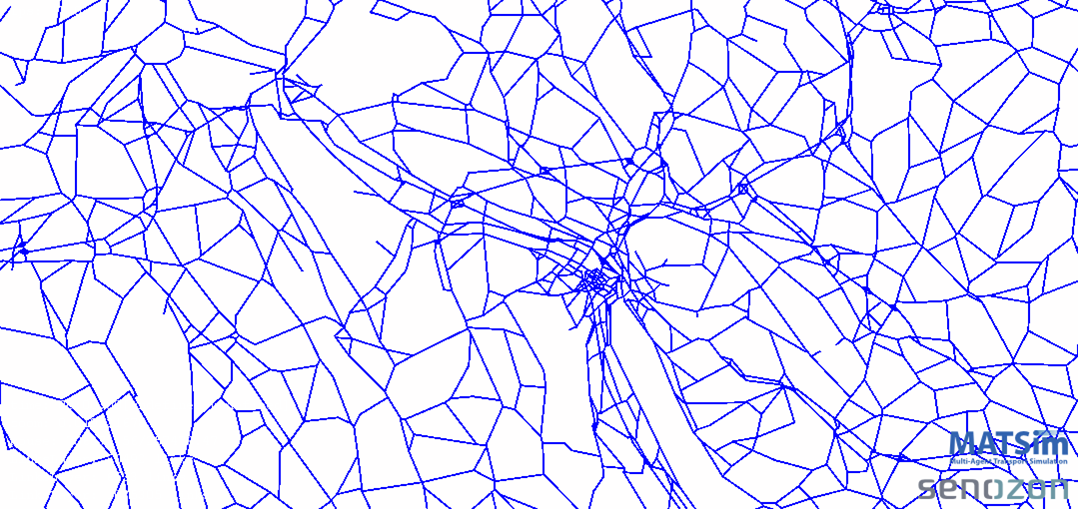
\includegraphics[width=0.8\textwidth,angle=0]{using/figures/planning.png}}%
  {\label{fig:planningnetwork}}%
  {}%
  \createsubfigure%
  {Navigation network}%
	{
\includegraphics[width=0.8\textwidth,angle=0]{using/figures/navigation.png}}%
  {\label{fig:navigationnetwork}}%
  {}%
}%
{}
%
In simulation practice, two different network types are used: planning networks and navigation networks (compare Swiss examples in Figure~\ref{fig:planningnetwork} and Figure~\ref{fig:navigationnetwork} for the Zürich region). The former are leaner and serve as initial explorative simulation runs, while the latter are used for policy runs, usually offering far more details, such as bike and even pedestrian links. Data are available from official sources like federal offices, free sources, such as \gls{osm}, and commercial sources, including navigation network providers.
%

\subsection{Example scenario input data}

Some example scenarios are included in the \gls{matsim} main distribution, in the directory ``examples''.

More pre-packaged scenarios can be found under \url{http://www.matsim.org/example-datasets}.

% ===============================================================================================
%\subsection{The Modeling Process: Implementation, Verification, Validation, and Calibration}
%\label{sec:using-modeling-process}
%
%%% \kai{Andreas, re Typographie: Es gibt die Theorie, dass Text bzgl.\ seiner ``grayness'' gleichmäßig aussehen sollte.  Daraus folgt, dass ``emph'' typischerweise Text in der gleichen ``Graustufe'' erzeugt wie normal. -- Ich persönlich habe es manchmal allerdings ganz gerne, wenn bestimmte Ausdrücke tatsächlich herausgehben sind ... wie im folgenden ``calibration'', ``verification'', ...  Bessere Lesbarkeit um den Preis der schlechteren Typographie.  Definiere dazu oft ``imp'', analog zu ``emph''.  Bin da allerdings nicht militant; wenn das einer Mehrheit nicht passt, ziehe ich mich hier zurück.}
%
%%% \ah{Finde ich gut. Einige "imp"s sind jetzt halt wieder rausgeflogen, wegen dem Einfügen von paragraphs.}
%
%% --------------------------------------
%\kai{Hallo Andreas,
%
%In Deinem Text plus dazugehörigem Bild steht, dass verification \emph{nach} calibration kommt.
%
%Ist das auch so in der originalen Quelle (Petty)?
%
%Ich hatte das immer umgekehrt gesehen.  Auch technisch machen wir es nahezu zwangsläufig umgekehrt: "verification" entspricht (meinem Verständnis nach) den regression tests, und die sind sinvollerweise im development process, und calibration kann erst danach kommen, nämlich wenn die user übernehmen.
%
%Auch \url{http://en.wikipedia.org/wiki/Verification_and_validation_of_computer_simulation_models} hat verification am Anfang; dort folgt interessanterweise gleich validation, und 
%calibration nur dann, wenn die validation scheitert (so würde ich das eigentlich auch sehen; wir haben in der Meteorologie nie kalibriert).
%
%Auch die NASA kennt nur verification und validation:  \url{http://www.grc.nasa.gov/WWW/wind/valid/tutorial/tutorial.html} .  (Calibration 
%wird dort im glossary genannt.)
%
%\url{http://www.streamnologies.com/support/pdfs/Calibration.pdf}
%hat verification \emph{nach} calibration ... verwechselt aber m.E. verification mit validation.
%
%\url{http://www.webpages.uidaho.edu/niatt_labmanual/chapters/traveldemandforecasting/professionalpractice/ModelCalibrationAndValidation.htm} : Verifying a calibrated model in this manner is commonly called "validation." :-)
%
%Viele Grüße
%
%Kai
%}
%
%% --------------------------------------
%\kai{Hallo Andreas,
%
%Nur schnell, ohne das genau gelesen zuhaben:
%
%verification -- software conforms to specifications
%
%validation -- software generates correct ``image'' of reality (gescheiterweise einschl. der sensitivities)
%
%calibration -- if validation fails (\ie an iterative cycle between validation and calibration)
%
%Also
%
%while ( validate()==false ) { 
   %calibrate() ; // if validate()==true immediately, this is never called }
%
%In den empirischen Sozialwissenschaften wird wohl davon ausgegangen, dass es ohne Kalibrierung ohnehin nicht validiert, daher
%
%do {
   %calibrate() ; // call at least once
%} until ( validate()==true ) ;
   %
%Ich selber tendiere allerdings (aufgrund Ausbildung?) auch dazu, erstmal ohne weitere Kalibrierung zu Validieren.
%
%===
%
%Da fällt mir allerdings gerade auf, dass die Verkehrsleute unter Kalibrierung etwas anderes Verstehen als die Naturwissenschaftler:
%
%- Ben-Akiva versteht unter Kalibrierung die upstream estimation des choice models. Also \emph{unabhängig} vom network loading model, traffic counts etc.  Er sagte mir sogar mal, "wenn alle Teil-Modelle richtig kalibriert sind, dann muss doch auch das Gesamt-Modell richtig kalibriert sein".
%
%- Meiner Erfahrung entspricht das nicht; das liegt an der Nicht-Linearität der ``emergent phenomena''.  Also muss man sich den Modell-Output anschauen, das Modell invertieren, und damit den Modell-Input (z.B. die Parameter der Nutzenfunktion) (nach)kalibrieren.  Das ist auch der Ansatz von Cadyts.
%
%Nun gut, müssen wir suchen.  Für die ``normale'' Sichtweise haben wir ja Perry und die NASA-webseite.  
%
%VG
%
%Kai
%}
%
%% --------------------------------------
%\kai{Figure 2: A scientific method to creating a model from a real world \[10\]:
%
%Kommentare:
%
%- ``verification'' (wo es wohl validation heißen müsste) --??
%
%- General solution --> Estimated real world: Hier wäre dann die ``calibration'' auch vor der validation.
%
%VG
%
%Kai
%}
%
%% --------------------------------------
%
%\kai{Go through text after above issue is resolved.}
%
%% =====================================================================
%
%Designing a \gls{microsimulation} scenario requires basic knowledge of the general modeling process, \ie a clear understanding of its required steps. 
%Thus, this section aims at giving the novice modeler a quick guide through the abstract modeling process. 
%The process is further detailed in Section~\ref{sec:extending-modeling-process} as it is particularly relevant for designing new functional modules, the topic of this book's part~II. 
%
%% ------------------------------------------------------
%\subsubsection{The Modeling Process in Theory}
%\label{sec:using-modeling-process-in-theory}
%The abstract modeling process is sketched in Figure~\ref{fig:modeling}---loosely based on \citet[][Figure 10.2]{Petty_SokolowskiBanks_2010}. 
%It starts with \imp{observation and measurement} of reality (in \citet[][]{Petty_SokolowskiBanks_2010} called ``\emph{simuland}'') for acquisition of \imp{knowledge} (in \citet[][]{Petty_SokolowskiBanks_2010} called ``\emph{referent}''). 
%\imp{Conceptual model} creation---in a strict sense, this is usually referred to as \emph{modeling}---is based on the modeler's knowledge about the world. 
%Based on a conceptual model, an \imp{executable model} is \imp{implemented}. 
%
%The executable model is evaluated in a \imp{verification} step in terms of ``\emph{was the model made right?}'' \citep[][p.332]{Petty_SokolowskiBanks_2010}, \ie verification is the procedure to test if a ``\emph{product is consistent with its specifications [...]}'' \citet[][p.330]{Petty_SokolowskiBanks_2010}. 
%In verification, a perfect match can be achieved between the conceptual and the executable model (see Figure~\ref{fig:modeling}) in contrast to validation (see below), where the model is always an approximation to reality \citep[][p.145]{Kleijnen_EJOR_1995}. 
%
%\imp{Validation} compares results with the referent in the sense of ``\emph{was the right model made?}'' \citep[][p.332]{Petty_SokolowskiBanks_2010}, \ie ``\emph{validation is the process of determining the degree to which the model is an accurate representation of the simuland.}'' \citep[][p.331]{Petty_SokolowskiBanks_2010}. 
%
%\imp{Calibration} is the process of adjusting model parameters to increase consistency of model outputs and observed target values \citep[][p.348]{HollanderLiu_Transportation_2007} \citep[see also][]{TrucanoEtAl_RESS_2006}. This is sometimes additionally necessary, when transferring a model from the domain it was built for to another---for example applying a social simulation for a different region. 
%
%% ----------
%\createfigure%
%{Modeling process}%
%{Modeling process}%
%{\label{fig:modeling}}%
%{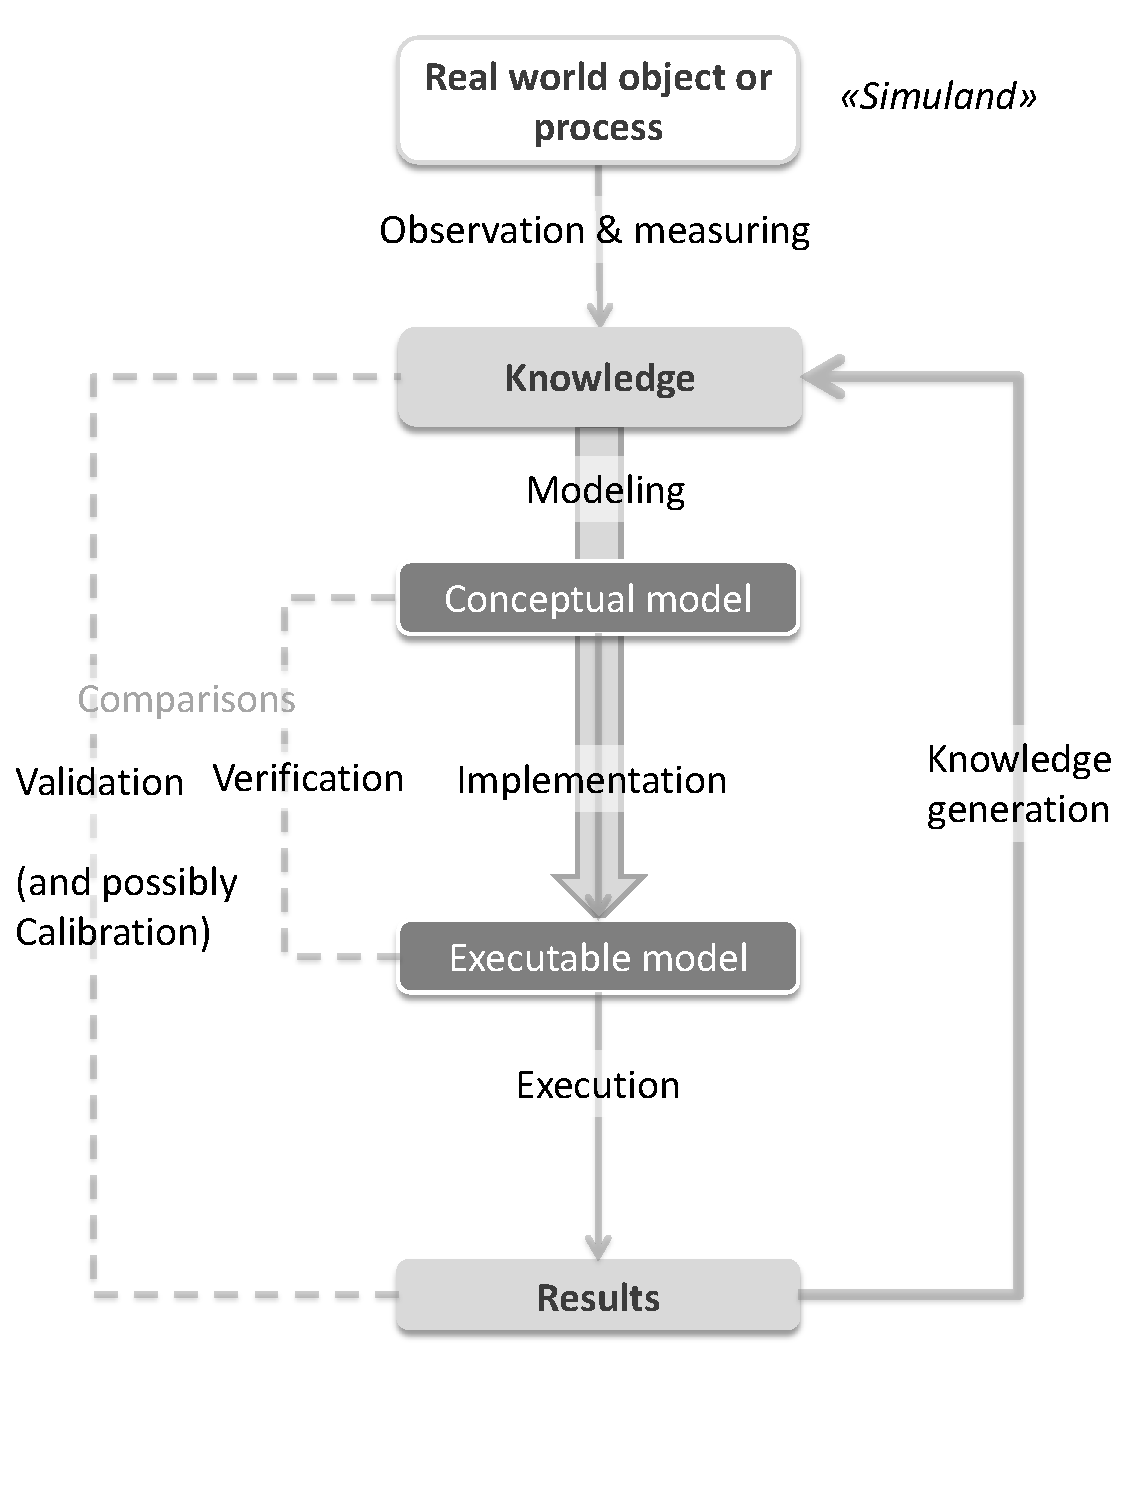
\includegraphics[width=0.8\textwidth, angle=0]{using/figures/modeling.pdf}}%
%{}
%% ----------
%
%% ------------------------------------------------------
%\subsubsection{The Modeling Process in Action in Transport Planning and MATSim}
%The modeling process as sketched above comes into play at two places: user's scenario creation, but also developer's simulator design. 
%Although, in this part of the book, the user is focused, here, we also consider the designer of new \gls{microsimulation} functionality as treated in part~II of the book.
%
%% ...................................................................
%\paragraph{Verification:}
%
%
%% ...................................................................
%\paragraph{Validation:}
%In practice, validation is difficult to standardize due to the variety of models and model purposes. 
%Some measures, tests, and applications relevant to transport modeling are given by \citet[][Table 2]{MilamChao_TRBATPM_2001}, \citet[][]{Lima_TechRep_LMPO_2006}, \citet[][p.155]{KurthEtAl_TRBTDF_2006}, \citet[][p.157]{PendyalaBhat_TRBTDF_2006}, \citet[][p.8]{WegmannEverett_TechRep_CTRUT_2008}, \citet[][]{MilamChao_TRBATPM_2001, RoordaEtAl_TransResA_2008, HawasHameed_TPT_2009, SadekEtAl_TRR_2003, GouliasKitamura_TRR_1992}, \citet[][p.25]{CambridgeSystematics_manual_2008}, \citet[][p.145]{Kleijnen_EJOR_1995} (see also \citet[][]{David_EACSSS_2009}, \citet[][p.56]{SbaytiRoden_ResRep_AASHTO_2010}, \citet[][]{SchifferRossi_TRB_2009}). 
%While for the 4-step procedure some validation standards have emerged \citep[e.g.,][]{BartonAschmanCambridgeSystematics_manual_1997}, a lack of standardization exists for activity-based models. 
%\citet[][]{PendyalaBhat_TRBTDF_2006} say that ``\emph{despite the appeal of these models,}'' [activity- and tour-based travel demand modeling systems] ``\emph{their widespread implementation appears to be hindered by the absence of a detailed validation and assessment of this new wave of model systems. 
%Many MPOs \ah{glossary} will not adopt such models until they are tested.}'' \citet[][]{KurthEtAl_TRBTDF_2006} cites a statement made by Chandra Bhat and Frank Koppelman in a DRCOG e-mail discussion: ``\emph{Researchers and practitioners have not thought carefully enough about the criteria for validation of models. 
%Researchers have the habit of asking practitioners to believe that activity- based methods will produce better impact assessment and forecasts because such models more appropriately represent the actual decision process (we plead guilty to this charge). There is a good basis for this line of thought, but researchers need to go beyond this argument. 
%They need to develop clear validation criteria and demonstrate the value of activity-based methods in ways that are easily understood.}''
%
%Often neglected, but important, is performing \imp{sensitivity analysis} (sometimes dubbed ``what-if analysis'' \citep[][p.155]{Kleijnen_EJOR_1995}) \citep[][]{KurthEtAl_TRBTDF_2006, CambridgeSystematics_manual_2008, CFD_TRB_2007}. 
%Sensitivity analysis is similar to assessing elasticity of a variable \citep[][p.3f]{WegmannEverett_TechRep_CTRUT_2008} and it tests reaction of the model to changed parameters including model input. 
%This includes both testing the range of parameters for a given point in time, and analysis of the system's fore- and backcasting abilities \citep[e.g.,][p.56]{CFD_TRB_2007}, \citep[][]{CambridgeSystematics_manual_2008}. 
%As forecasting is a vital objective of most transport models, this test is crucial. 
%\citet[][p.158]{PendyalaBhat_TRBTDF_2006} puts it succinctly: ``\emph{There is no doubt that any model can be adjusted, refined, tweaked, and---if all else fails---hammered to replicate base-year conditions.}'' and concludes that ``\emph{the quality of a travel demand model system is better judged on its ability to respond to a range of scenarios and policies of interest.}''
%
%In \gls{matsim}, a natural and interesting sensitivity test would be to compare the \gls{matsim} forecasts with the current actual state of Zürich network after addition of the bypass ``Westumfahrung'' in 2009 \citep[][]{Westumfahrung_Webpage_2008}, researched in detail by \citet[][]{BalmerEtAl_ResRep_bdktzrh_2009}.
%
%% ...................................................................
%\paragraph{Calibration:}
%\citet[][Table 1]{HollanderLiu_Transportation_2007} list numerous studies that each calibrate a specific transport \gls{microsimulation}. Further examples are \citet[][]{SmithEtAl_JTE_2008, KimEtAl_TRR_2005, RutterEtAl_JASA_2009}, \gls{microsimulation} calibration guidelines are provided by \citet[][]{MilamChao_TRBATPM_2001, WegmannEverett_TechRep_CTRUT_2008, DowlingEtAl_manual_2002}. \citet[][Table 2]{HollanderLiu_Transportation_2007} describe measures of goodness-of-fit, that are productive for calibration. 
%
%The main calibration component for \gls{matsim} is the \gls{utilityfunction}; it needs to reflect the preferences of the study area's population.
%
%A second prominent calibration screw is in particular used for sample runs: To reduce the computational effort, initial explorative simulation runs are often performed on samples of the full population. In this case, either the flow and storage capacity values of the mobility simulation or the network capacities need to be adapted accordingly. \kai{described where?}
%
%Due to the usually large number of model parameters, an automated process is favorable as far as possible. 
%Essentially this is an optimization process \citep[][p.353]{HollanderLiu_Transportation_2007}, for which various established procedures exist \citep[e.g.,][p.41ff]{ZhangMa_ResRep_PATH_2008}. 
%For \gls{matsim}, an automatic procedure adapting the plans to road counts was developed by \citet[][]{floetteroed-2010e}. 
%It is unclear however, if a certain loss of behavioral soundness is caused by adapting plans according to statistical matching. On the other hand, it is unclear anyway, to date, if the \gls{matsim} relaxation transitions should be given a behavioral meaning. 
%
%% ...................................................................
%
%As mentioned above, models are in general flexible enough to be calibrated to target data. Thus, validation \emph{must} be performed using a different data set than for creating or calibrating the model \citep[][p.1]{CambridgeSystematics_manual_2008}, \citep[][p.56]{CFD_TRB_2007}, \citep[][p.18]{OrtuzarWillumsen_2001}. In statistics, this is called cross-validation. It is particularly important for forecasting models, which need to be general enough to capture temporal changes. Calibration and validation should thus be strictly separated. Due to the vast amount of data required for model implementation and calibration this is not an easy endeavor for \gls{microsimulation} practice. In \gls{matsim}, for example, after model creation often only road count data is left for validation \citep[][]{HorniEtAl_STRC_2009}. New data sources, such as road speed analyses based on \gls{gps} \citep[][]{HackneyEtAl_JGS_2007}, should be included.
%
%Furthermore, many central and comfortable characteristics of systems known from natural sciences are only seldom available for the social science, such as path-independence, decomposability, isolation, and on top of that repeatability of experiments. As a result, there is still a debate if social science actually can provide something similar as laws. \citet[][p.107ff]{Abel_1976} lists and discusses the 12\,claims of the ``\emph{Verstehen Position}''; although, he finds contrary arguments to every claim, nevertheless, something definitely remains true, making social science model validation exceptionally difficult. 
%
%Verification and validation, are of more concern for the \gls{microsimulation} developers. Given a valuable estimate for demand and supply including a properly estimated utility function, from customer's perspective the simulation can be expected to generate valuable single run results out of the box for the design domain.
%
%Besides possibly calibrating the model for different application domains, the user's or customer's responsibility is asked, at another place: \Glspl{microsimulation} are basically a sampling tool, just as a survey (see Section~\ref{sec:variability}). A single run represents the sampling unit, the individual in surveys. This obviously means that \gls{microsimulation} results must not to be presented as single runs but with the help of the usual statistical tools, \eg by parameters with the common measures of spread or confidence intervals. That basically means that the user/customer is responsible to specify the sample size, the number of simulation runs initialized with different random seeds. 
%
%%Policy evaluations are often based on count data, usually widely available but also showing substantial temporal variability. For \gls{matsim}, the count data need to be converted to match the simulated period of the day.
%
%%\ah{Latte zu hoch gelegt und wohl gerissen:}
%%For microsimulation results interpretation and model validation, it helps to visualize the following example. A microsimulation forecast (or backcast) regarding the construction of the "Westumfahrung Zürich" provides a probability distribution of scenarios, and it is essentially an exercise in Monte Carlo sampling (see also Chapter~\ref{ch:montecarlo}). 4\,years later we have exactly one actual state, and there is no way to assess the forecasted (or backcasted) probability distribution beyond checking that this actual state is contained in the probability distribution, and hopefully with high probability. There is nothing like Monte Carlo sampling when it comes to aggregate real system states. In other words the existing state is \emph{unique}. In essence, we thus compare an observed Dirac impulse with a computed probability distribution, which is a difficult undertaking.

% ##################################################################################################################
\section{MATSim Survival Guide}
\label{sec:survival}

%% \kai{Wenn wir in Teil I hinter ``scoring'' noch ein Kapitel bauen, welches sozusagen ``configurations which are not extensions'' enthält, dann könnte survival guide an dessen Ende. (??)}

%% \ah{Chapter~\ref{ch:configuring}, ist momentan vor Scoring. Finde den MATSim Survival Guide hier eigentlich auch ganz passend.}

%ok dann bleibt er hier. kai, jan'15

There are many options and possibilities available with \gls{matsim}, and finding them can be a taunting exercise.  Here are a couple of recommendations, derived from our own frequent use of the system.
\begin{enumerate}\styleEnumerate

\item \emph{Always start and test with a small example.}

\item \emph{Always test large scenarios with one percent runs first (\eg a randomly drawn a 10\,\% or a 1\,\% subsample of your initial demand).} The \gls{matsim} \gls{gui} (Figure~\ref{fig:matsimgui}) allows to create sample populations with the command \lstinline|Tools...Create Sample Population|.

As described in Section~\ref{sec:using-mobsims}, this requires adaptation of parameters, in particular the \gls{mobsim}'s \lstinline|flowCapacityFactor| and \lstinline|storageCapacityFactor| factors. As shown in part~II of the book, in Section~\ref{sec:extending-counts}, sample scenarios also require parameter adaption for count data comparisons. %The \gls{matsim} \gls{gui} (Figure~\ref{fig:matsimgui}) allows to adapt all parameters at once with the command \lstinline|Tools...Create Sample Population|. %\ah{thx Marcel! :)}

%% \kaitodo{this needs to be described somewhere.  flowcap; storcap larger (see matsim4urbansim); counts [[this todo got commented out, but withouth description of what was done ... for example, in matsim4urbansim, we set storage capacity to something like $1/sampleSize^{0.25}$ including documentation for this; is this done here as well?]]}

%\ahtodo{\kai{Andreas, I just checked the code, and it does not look like it is doing antying but creating the sample population.  (And write it to a separate file, which can then be used together with a different config file.)  Where does the info come from that it also adapts config parameter values?}}

%\ah{Weiss ich leider nicht mehr. Aber klingt danach als hätte ich es irgendwo gelesen.}

\item \emph{If your set-up does not work any more, \emph{immediately} go back to a working version and proceed from there in small steps.}

\item \emph{Check \lstinline{logfileWarningors.log}.}

\item \emph{Check the comments that are attached to the \gls{configfile} options.}

One finds them in the file \lstinline{output_config.xml.gz}, or near the beginning of \lstinline{logfile.log}.

\item \emph{Try setting as few \gls{configfile} options as possible.}

This has two advantages: (i) Except for the deliberately set options, your simulation will move along with changed \gls{matsim} defaults, and thus with what the community currently considers the best configuration.  (ii) You will not be affected by changes in the \gls{configfile} syntax as long as the are different from your own settings.

\item \emph{Search for documentation via \url{http://matsim.org/javadoc}.}

\end{enumerate}

  %\kai{Andreas, finde es problematisch, den itemsep kleiner zu haben als den itemskip (oder ist das parskip?).  Dann sieht es aus wie in item 5 oben.  Würde aber sehr dafür plädiren, den itemsep nach oben zu setzen; finde, dass es die Lesbarkeit deutlich verschlechtert, wenn zwischen den items gar kein Abstand ist.}
%\ah{ist korrigiert. itemsep vs. parsep. Neues Package ``enumitem'' verwendet.}

% ##################################################################################################################
\ifthenelse{\boolean{printBibPerChapter}}{\bibpc}{}

% ##################################################################################################################

% Local Variables:
% mode: latex
% mode: reftex
% mode: visual-line
% TeX-master: "../main"
% comment-padding: 1
% fill-column: 9999
% End: 
